\documentclass[acmsmall,screen,dvipsnames,x11names,nonacm,anonymous,review]{acmart}
\usepackage[most]{tcolorbox}
\usepackage{listings}
\usepackage{caption}
\usepackage{cleveref}
% Redefine sections to display with § symbol
\crefformat{section}{\S#2#1#3}
\Crefformat{section}{\S#2#1#3}

% Ensure subsections/subsubsections behave the same way (optional)
\crefformat{subsection}{\S#2#1#3}
\Crefformat{subsection}{\S#2#1#3}
\crefformat{subsubsection}{\S#2#1#3}
\Crefformat{subsubsection}{\S#2#1#3}

\usepackage[table,xcdraw]{xcolor}
\usepackage{tikz}
\definecolor{col1}{HTML}{90f1ef}
\definecolor{col2}{HTML}{ffd6e0}
\definecolor{col3}{HTML}{ffef9f}

\definecolor{typecolor}{HTML}{4169E1} % RoyalBlue
\newcommand{\codetype}[1]{\textcolor{typecolor}{\ttfamily\small#1}}
% Macros for float type notation with proper braces
% Use \ftb{bounds}{values} for float type with both bounds and values
% Use \ft{bounds} for float type with bounds and T for values
% Use \ftt for float[T; T]
\newcommand{\ftb}[2]{\codetype{float[\{#1\}; \{#2\}]}}  % Both bags have values
\newcommand{\ft}[1]{\codetype{float[\{#1\}; T]}}        % Bounds only, values are T
\newcommand{\ftt}{\codetype{float[T; T]}}               % Both bags are T
\newcommand{\ftv}[1]{\codetype{float[T; \{#1\}]}}       % Bounds are T, values specified

\renewcommand{\paragraph}[1]{\vspace{1em}\noindent\textbf{#1}\ }

\newcommand{\alexandra}[1]{\textcolor{pink}{\textbf{Alexandra:} #1}}
\newcommand{\kevin}[1]{\textcolor{ForestGreen}{\textbf{Kevin:} #1}}
\newcommand{\katherine}[1]{\textcolor{Purple}{\textbf{Katherine:} #1}}
\newcommand{\jules}[1]{\textcolor{blue}{\textbf{Jules:} #1}}




\tcbuselibrary{listingsutf8}

\newtcblisting{mybox}[2][]{%
  colback=#2!20,
  colframe=#2!80!black,
  coltitle=white,
  boxrule=1pt,
  arc=6pt,
  fonttitle=\bfseries\footnotesize,
  listing only,
  listing options={
    basicstyle=\ttfamily\footnotesize,
    breaklines=true,
    language=Dice,
    showstringspaces=false
  },
  width=\linewidth,
  valign=top,
  height=3.6cm,
  #1
}
\usepackage[scaled=0.84]{beramono}
\usepackage{mathpartir}
\usepackage{xspace}
\usepackage{todonotes}
\usepackage{subcaption}
\title{Slice: Type-Directed Discretization of Continuous Probabilistic Programs}

\lstdefinelanguage{Dice}{
    morekeywords={let, in, if, then, else, fst, snd, fun},
    morekeywords=[2]{uniform, discrete, gaussian, exponential, beta},
    morekeywords=[3]{bool, float, int},
    basicstyle=\ttfamily\small,
    keywordstyle=\bfseries,
    commentstyle=\itshape,
    stringstyle=\ttfamily,
    lineskip=-1pt,                
    aboveskip=0.1em,                
    belowskip=0.1em,
}




% Macros for language keywords to be used in math mode
\newcommand{\letkw}{\text{\ttfamily\bfseries let}}
\newcommand{\inkw}{\text{\ttfamily\bfseries in}}
\newcommand{\ifkw}{\text{\ttfamily\bfseries if}}
\newcommand{\thenkw}{\text{\ttfamily\bfseries then}}
\newcommand{\elsekw}{\text{\ttfamily\bfseries else}}
\newcommand{\uniform}{\text{\ttfamily\bfseries uniform}}
\newcommand{\discrete}{\text{\ttfamily\bfseries discrete}}
\newcommand{\gaussian}{\text{\ttfamily\bfseries gaussian}}
\newcommand{\exponential}{\text{\ttfamily\bfseries exponential}}
\newcommand{\betafn}{\text{\ttfamily\bfseries beta}} % Use beta for the keyword
\newcommand{\fstkw}{\text{\ttfamily\bfseries fst}}
\newcommand{\sndkw}{\text{\ttfamily\bfseries snd}}
\newcommand{\funkw}{\text{\ttfamily\bfseries fun}}
\newcommand{\bool}{\text{\ttfamily\bfseries bool}}
\newcommand{\intty}{\text{\ttfamily\bfseries int}}
\newcommand{\float}{\text{\ttfamily\bfseries float}}

% Macros for language names, use small caps
\newcommand{\Slice}{\text{\scshape Slice}\xspace}
\newcommand{\Dice}{\text{\scshape Dice}\xspace}

\newcommand{\R}{\mathbb{R}}

% Set this as the default language for listings
\lstset{language=Dice}

\begin{document}

\begin{abstract}
Probabilistic programming languages are a powerful tool for statistical modeling, but performing exact inference on programs with continuous random variables remains a major challenge. This paper presents \Slice{}, a language that enables exact inference for a broad class of programs with continuous distributions. \Slice{} works by automatically and soundly discretizing continuous variables. The core of our approach is a novel type system that analyzes how continuous random variables are compared within a program. It uses this information to partition the continuous domains into a finite number of intervals, transforming the original program into an equivalent, purely discrete one. This transformed program can then be solved by a backend exact inference engine for discrete PPLs. We formalize this type-directed discretization, prove its soundness, and provide an open-source implementation. Our evaluation shows that our approach is significantly faster than existing symbolic inference techniques for hybrid discrete-continuous programs, bridging the gap between expressive continuous modeling and the power of exact discrete inference.
\end{abstract}

\maketitle

\section{Introduction}\label{sec:intro}
Probabilistic programming languages have emerged as a powerful tool for building complex statistical models and reasoning about uncertainty~\cite{Moy2025Roulette,Holtzen2020Dice,DeRaedt2007ProbLog,Saad2021SPPL,Carpenter2017Stan,Salvatier2016PyMC3,Bingham2019Pyro,Dillon2017TFP,Tran2016Edward,Tolpin2016Anglican,Goodman2014WebPPL,Pfeffer2009Figaro,Minka2018InferNET,Ge2018Turing,CusumanoTowner2019Gen,Tehrani2020BeanMachine,Goodman2008Church}. A key challenge in PPLs is inference: computing the probability of an event given a model. The tractability of inference often depends on the kinds of random variables used. For programs with only discrete random variables, powerful exact inference engines can compute probabilities precisely. However, many real-world models require continuous random variables to represent quantities like time, distance, or sensor readings. For these programs, exact inference is often intractable, forcing practitioners to rely on approximate methods like Monte Carlo simulation or variational inference. 

Existing discrete PPLs like \Dice~\cite{Holtzen2020Dice} and Roulette~\cite{Moy2025Roulette} offer powerful, exact inference but cannot handle continuous distributions. At the other end of the spectrum, popular general-purpose PPLs like Stan~\cite{Carpenter2017Stan} and Pyro~\cite{Bingham2019Pyro} excel at approximate inference for continuous models but sacrifice exactness. Symbolic inference systems like SPPL~\cite{Saad2021SPPL} can reason exactly about certain mixed discrete-continuous models.

This paper introduces \Slice{}, which occupies a unique position in the PPL design space: it automatically and soundly translates a broad class of programs with continuous variables into equivalent discrete programs. This automated, sound discretization unlocks the ability to use powerful discrete exact inference engines on models that were previously out of their reach. The key insight is to analyze how continuous variables are used within the program. Specifically, \Slice{} uses a type system to track all the constant thresholds against which continuous variables are compared. These comparison points are then used to intelligently discretize the continuous distributions into a finite number of buckets. When the resulting program is purely discrete it can then be solved by an off-the-shelf exact inference engine such as Dice~\cite{Holtzen2020Dice}. This type-directed discretization allows developers to model with continuous distributions while still benefiting from the speed and precision of exact discrete inference.

Consider the simplest possible example---checking if a uniform random variable is less than 0.5:

\begin{lstlisting}[aboveskip=1em,belowskip=1em]
    uniform(0, 1) < 0.5
\end{lstlisting}

\noindent \Slice{} automatically transforms this into:

\begin{lstlisting}[aboveskip=1em,belowskip=1em]
    discrete(0.5, 0.5) < 1
\end{lstlisting}

\noindent The uniform distribution is replaced by a discrete distribution with two equally likely outcomes, and the comparison is adapted accordingly. Here is a more complex example:

\begin{lstlisting}[aboveskip=1em,belowskip=1em]
    let x = uniform(0, 1) in
    let y = uniform(0, 2) in
    if x < 0.5 then x < 0.1 else y < 0.1
\end{lstlisting}

\noindent The program above can be discretized into:

\begin{lstlisting}[aboveskip=1em,belowskip=1em]
    let x = discrete(0.1, 0.4, 0.5) in
    let y = discrete(0.05, 0.95) in
    if x < 2 then x < 1 else y < 1
\end{lstlisting}

The discretization process is driven by the comparisons present in the program. \Slice{} analyzes the program to find all numeric constants used in comparisons with continuous random variables. In the example above, the variable \texttt{x}, drawn from a \texttt{uniform(0, 1)} distribution, is compared to 0.5 and 0.1. These two ``split points'' partition the range of \texttt{x} into three intervals: $(-\infty, 0.1)$, $[0.1, 0.5)$, and $[0.5, +\infty)$. \Slice{} replaces the continuous distribution for \texttt{x} with a discrete one that has three outcomes, where the probability of each outcome is equal to the probability mass of the original uniform distribution within the corresponding interval. Similarly, the variable \texttt{y}, drawn from \texttt{uniform(0, 2)}, is compared only to 0.1, partitioning its distribution into two intervals. All comparisons are then transformed to operate on these new discrete variables. This example illustrates the core mechanism of \Slice{}: a type-directed transformation that makes continuous programs amenable to exact discrete inference.

\jules{TODO: add a paragraph about which language features are supported in Slice.}

\paragraph{Contributions.}

We first introduce \Slice{} through examples (\Cref{sec:examples}), and then present and evaluate our framework for type-directed discretization via the following contributions:

\begin{description}
    \item[Type System (\Cref{sec:language})] We introduce a novel type system that identifies which expressions are discretizable based on how they are used throughout the program.

    \item[Type Inference (\Cref{sec:type-inference})] We develop a type inference algorithm that automatically collects the set of constant thresholds needed for discretization for each expression.

    \item[Discretization (\Cref{sec:discretization})] We present a type-directed transformation that soundly converts continuous distributions and their comparisons into discrete counterparts. We characterize the class of programs for which this transformation results in a fully discrete program.

    \item[Soundness (\Cref{sec:soundness})] We prove that our discretization method is sound, establishing that the discretized program preserves the semantics of the original program.

    \item[Implementation (\Cref{sec:implementation})] We provide an open-source implementation of our system, \Slice{}. The system transforms a given \Slice{} program into another, more discretized \Slice{} program. If the resulting program is fully discrete, it can be compiled for the \Dice{} probabilistic programming system to leverage its highly-optimized exact inference engine. We have also implemented a direct Monte Carlo simulator for \Slice{} itself, which can handle any program, including those that are only partially discretized.

    \item[Evaluation (\Cref{sec:evaluation})] We conduct a thorough empirical evaluation of our approach on a range of benchmarks, including those used to evaluate existing systems like SPPL\@. The results show that our method of discretization followed by exact discrete inference is significantly faster than prior symbolic techniques, while maintaining the same level of correctness.
\end{description}

\section{Slice by Example}\label{sec:examples}
This section presents simple examples that highlight the key features of our probabilistic programming language \Slice{}, aiming to emphasize how \Slice{} meets the challenge of performing exact inference efficiently. \Slice{} extends a core functional language with traditional programming language constructs such as conditionals, local variables, and functions, augmented with constructs for probabilistic programming such as sampling and conditioning. Each example in the subsections is intended to showcase these features. Later in the section, we also mention examples that can only be partially discretized but nonetheless preserve the semantics across both the original and discretized program.

\subsection{Simple branching on a uniform distribution}

We start with a simple example that illustrates the core idea of \Slice{}. Consider the following program, which models a fair coin flip by checking if a random number from a uniform distribution is less than 0.5:

\begin{lstlisting}[aboveskip=1em,belowskip=1em]
    uniform(0,1) < 0.5
\end{lstlisting}

\noindent \Slice{}'s type system analyzes this program and identifies that the only comparison point for the continuous variable is 0.5. This single split point partitions the range $\R = (-\infty, +\infty)$ into two intervals of equal probability mass: $(-\infty, 0.5)$ and $[0.5, +\infty)$. \Slice{} then transforms the program into an equivalent discrete version:

\begin{lstlisting}[aboveskip=1em,belowskip=1em]
    discrete(0.5, 0.5) < 1
\end{lstlisting}

\noindent Here, \texttt{discrete(0.5, 0.5)} represents a choice between two outcomes (0 or 1), each with probability 0.5. The outcome 0 corresponds to the original value being in $(-\infty, 0.5)$, and 1 corresponds to it being in $[0.5, +\infty)$. The comparison is updated to check if the outcome is less than 1, which is true only for outcome 0, correctly preserving the original program's meaning. This transformation is guided by tracking comparison points, which are determined by type inference as shown in the annotated program below:

\begin{lstlisting}[aboveskip=1em,belowskip=1em,escapechar=!]
    (uniform(0, 1) : !{\ft{<0.5}}!) < (0.5 : !{\ftb{<0.5}{0.5}}!)
\end{lstlisting}

The type \ft{<0.5} for the uniform sample indicates that the bound bag contains the comparison bound ``$<\!\!0.5$'' and the value bag is $\top$ (can take any value in the range). 
The type \ftb{<0.5}{0.5} for the constant $0.5$ indicates that the bound bag contains $<0.5$ and the value bag contains only the single value $0.5$.

In general, a type \lstinline{float[bound-bag; value-bag]} indicates:
\[
\textbf{float}
[
\underbrace{\text{bound-bag}}_{\begin{array}{c}\text{set of comparison bounds}\\\text{(e.g., }\{<\!0.1, <\!0.5, \leq\!0.8\}\text{)}\\\text{or }\top\text{ (unbounded)}\end{array}}
;
\underbrace{\text{value-bag}}_{\begin{array}{c}\text{set of concrete values}\\\text{(e.g., }\{0.1, 0.4, 0.5\}\text{)}\\\text{or }\top\text{ (any value)}\end{array}}
]
\]

The bound bag is determined by \emph{how the expression is used} (i.e., what it's compared against) and the value bag is determined by \emph{what concrete values the expression can take}.
The discretization is driven by the bound bag: a float value with $n$ comparison bounds is discretized into $n+1$ possible discrete values.

In the example above, the expression \lstinline{uniform(0,1)} is discretized to \lstinline{discrete(0.5, 0.5)} which returns $0$ with probability $0.5$ and $1$ with probability $0.5$.
The constant $0.5$ on the right hand side is discretized to the constant $1$ because it falls in the second range $[0.5, +\infty)$. The less-than comparison is translated to an identical less-than comparison on the discrete values.

\subsection{Branching on multiple continuous variables}

\noindent Now let's consider a more complex example with multiple continuous variables and conditional branches:

\begin{lstlisting}[aboveskip=1em,belowskip=1em]
    let x = uniform(0, 1) in
    let y = uniform(0, 2) in
    if x < 0.5 then x < 0.1 else y < 0.1
\end{lstlisting}

\noindent In this program, the variable \texttt{x} is drawn from \texttt{uniform(0, 1)} and is compared against two different constants: \texttt{0.5} and \texttt{0.1}. These two cut points partition the real line $\R$ into three intervals: $(-\infty, 0.1)$, $[0.1, 0.5)$, and $[0.5, +\infty)$. Similarly, the variable \texttt{y}, drawn from \texttt{uniform(0, 2)}, is compared only with \texttt{0.1}. This single cut point partitions the real line $\R$ into two intervals, $(-\infty, 0.1)$ and $[0.1, +\infty)$.


This analysis is done by the type inference process, which collects all comparison points for each continuous variable. For \texttt{x}, the type inference algorithm discovers the cut points \texttt{<0.1} and \texttt{<0.5}, giving it the type \ft{<0.1,<0.5}. For \texttt{y}, it only finds \texttt{<0.1}, giving it the type \ft{<0.1}. This information is captured in the annotated program below.

\begin{lstlisting}[aboveskip=1em,belowskip=1em,escapechar=!]
    let x = uniform(0, 1) : !{\ft{<0.1,<0.5}}! in
    let y = uniform(0, 2) : !{\ft{<0.5}}! in
    if x < (0.1 : !{\ftb{<0.1,<0.5}{0.1}}!) then
      x < (0.5 : !{\ftb{<0.1,<0.5}{0.5}}!)
    else
      y < (0.5 : !{\ftb{<0.5}{0.5}}!)
\end{lstlisting}


\Slice{} replaces the continuous distribution for \texttt{x} with a discrete one that has three outcomes, where the probability of each outcome is the probability mass of the original uniform distribution within the corresponding interval. This results in \texttt{discrete(0.1, 0.4, 0.5)}.
\Slice{} replaces the continuous distribution for \texttt{y} with a discrete one that has two outcomes, where the probability of each outcome is the probability mass of the original uniform distribution within the corresponding interval. This results in \texttt{discrete(0.05, 0.95)}. The comparisons in the program are then transformed to operate on the integer indices of these new discrete intervals, leading to the following discretized program:

\begin{lstlisting}[aboveskip=1em,belowskip=1em]
    let x = discrete(0.1, 0.4, 0.5) in
    let y = discrete(0.05, 0.95) in
    if x < 1 then
      x < 2
    else
      y < 1
\end{lstlisting}

Note that the original constant $0.5$ is discretized in two different ways: for $x < 0.5$ it is discretized to $2$ and for $y < 0.5$ it is discretized to $1$. This is because the constant $0.5$ falls in the second interval of the split $\R = (-\infty, 0.1) \cup [0.1, 0.5) \cup [0.5, +\infty)$ for $x$ and the first interval for the split $\R = (-\infty, 0.5) \cup [0.5, +\infty)$ for $y$.

\subsection{If else with continuous values}

In the program above, we always directly compare the continuous samples to constants.
However, the discretization process still works if the continuous samples and constants flow through the program, for instance via an if-else statement.
Consider the following program:

\begin{lstlisting}[aboveskip=1em,belowskip=1em,escapechar=!]
    let x = if uniform(0,1) < 0.5 
            then uniform(0,2) 
            else gaussian(0,1) in
    let y = if 1.5 < x
            then 1.8
            else 0.3 in
    x <= y
\end{lstlisting}

\noindent This program demonstrates how comparison points propagate through control flow. The type inference annotates the program as follows:

\begin{lstlisting}[aboveskip=1em,belowskip=1em,escapechar=!]
    let x = if (uniform(0,1) : !{\ft{<0.5}}!) < (0.5 : !{\ftb{<0.5}{0.5}}!)
            then (uniform(0,2) : !{\ft{<=0.3,<1.5,<=1.8}}!)
            else (gaussian(0,1) : !{\ft{<=0.3,<1.5,<=1.8}}!)
            : !{\ft{<=0.3,<1.5,<=1.8}}! in
    let y = if (1.5 : !{\ftb{<=0.3,<1.5,<=1.8}{1.5}}!) < x
            then (1.8 : !{\ftb{<=0.3,<1.5,<=1.8}{1.8}}!)
            else (0.3 : !{\ftb{<=0.3,<1.5,<=1.8}{0.3}}!)
            : !{\ftb{<=0.3,<1.5,<=1.8}{0.3,1.8}}! in
    x <= y
\end{lstlisting}

\noindent Notice that all comparison points from the entire program (0.3, 1.5, and 1.8) are collected for the variable \texttt{x}, regardless of which branch is taken. These comparison points with type \codetype{<=0.3,<1.5,<=1.8} split the real line into four intervals: $(-\infty, 0.3]$, $(0.3, 1.5)$, $[1.5, 1.8]$, and $(1.8, +\infty)$. Note that 1.5 is excluded from the second interval and included in the third because it comes from a strict `<` comparison. The discretized version becomes:

\begin{lstlisting}[aboveskip=1em,belowskip=1em]
    let x = if discrete(0.5, 0.5) < 1 then
        discrete(0.15, 0.6, 0.15, 0.1)
      else
        discrete(0.617911, 0.315281, 0.0308769, 0.0359303) in
    let y = if 1 < x then 2 else 0 in
    x <= y
\end{lstlisting}

\noindent The four probabilities in each \texttt{discrete} distribution correspond to the probability mass in each of the four intervals. For example, \texttt{uniform(0,2)} has probability 0.15 in $(-\infty, 0.3]$, 0.6 in $(0.3, 1.5]$, 0.15 in $(1.5, 1.8]$, and 0.1 in $(1.8, +\infty)$.

\subsection{Discrete latent variable}

Continuous distributions can have parameters that depend on discrete random choices. In this example, a Gaussian distribution's standard deviation is determined by a random choice between two values:

\begin{lstlisting}[aboveskip=1em,belowskip=1em,escapechar=!]
    let x = if uniform(0,1) < 0.5 
            then 0.5
            else 1.5 in
    gaussian(0, x) < 0.5
\end{lstlisting}

\noindent This example shows how discrete choices can affect the parameters of continuous distributions. The type-annotated version reveals how the discrete latent variable \texttt{x} determines the standard deviation of the Gaussian:

\begin{lstlisting}[aboveskip=1em,belowskip=1em,escapechar=!]
    let x = if (uniform(0,1) : !{\ft{<0.5}}!) < (0.5 : !{\ftb{<0.5}{0.5}}!)
            then (0.5 : !{\ftb{<=0.5,<=1.5}{0.5}}!)
            else (1.5 : !{\ftb{<=0.5,<=1.5}{1.5}}!)
            : !{\ftb{<=0.5,<=1.5}{0.5,1.5}}! in
    (gaussian(0, x) : !{\ft{<0.5}}!) < (0.5 : !{\ftb{<0.5}{0.5}}!)
\end{lstlisting}

\noindent The discretized program handles the distribution parameter that depends on a discrete choice:

\begin{lstlisting}[aboveskip=1em,belowskip=1em]
    let x = if discrete(0.5, 0.5) < 1 then 0 else 1 in
    (if x == 0 then
        discrete(0.841345, 0.158655)
    else
        discrete(0.630559, 0.369441)) < 1
\end{lstlisting}

\subsection{Conditioning}

\Slice{} supports conditioning on events through the \texttt{observe} construct, allowing for Bayesian inference. The following program computes the probability that a uniform random variable is less than 0.2, given that it is less than 0.5:

\begin{lstlisting}[aboveskip=1em,belowskip=1em,escapechar=!]
    let x = uniform(0.0, 1.0) in
    observe (x < 0.5);
    x < 0.2
\end{lstlisting}

\noindent The type-annotated version shows how observation points become comparison points:

\begin{lstlisting}[aboveskip=1em,belowskip=1em,escapechar=!]
    let x = (uniform(0.0, 1.0) : !{\ft{<0.2,<0.5}}!) in
    observe (x < (0.5 : !{\ftb{<0.2,<0.5}{0.5}}!));
    x < (0.2 : !{\ftb{<0.2,<0.5}{0.2}}!)
\end{lstlisting}

\noindent The discretized version preserves the conditioning semantics:

\begin{lstlisting}[aboveskip=1em,belowskip=1em]
    let x = discrete(0.2, 0.3, 0.5) in
    observe (x < 2);
    x < 1
\end{lstlisting}

\noindent In the discrete version, the observation \texttt{x < 2} rules out the case where \texttt{x = 2} (corresponding to the original interval $[0.5, +\infty)$), effectively conditioning on \texttt{x} being in $[0.0, 0.5)$.

\subsection{Higher-order functions}

\Slice{} supports higher-order functions, enabling functional programming patterns with probabilistic computations. This example shows a higher-order function \texttt{mappair} that applies a function to both elements of a pair:

\begin{lstlisting}[aboveskip=1em,belowskip=1em,escapechar=!]
  let mappair = fun f -> fun p -> (f (fst p), f (snd p)) in
  let f = fun x -> x < 0.5 in
  let g = fun x -> x < 1.5 in
  let p = (uniform(0,2), gaussian(0,2)) in
  let q = (mappair f) p in
  let r = (mappair g) p in
  if fst q then snd q else 
      if fst r then snd r else fst q
\end{lstlisting}

\noindent The type system correctly infers that comparison points from both \texttt{f} and \texttt{g} (0.5 and 1.5) must be collected for the distributions in \texttt{p}, yielding type \ft{<0.5,<1.5} for both components. The discretized version preserves the higher-order structure:

\begin{lstlisting}[aboveskip=1em,belowskip=1em]
  let mappair = fun f -> fun p -> (f (fst p), f (snd p)) in
  let f = fun x -> x < 1 in
  let g = fun x -> x < 2 in
  let p = (discrete(0.25, 0.5, 0.25), 
          discrete(0.598706, 0.174666, 0.226627)) in
  let q = (mappair f) p in
  let r = (mappair g) p in
  if fst q then snd q else 
      if fst r then snd r else fst q
\end{lstlisting}

\noindent The continuous distributions are discretized into three-valued discrete distributions based on the intervals $(-\infty, 0.5)$, $[0.5, 1.5)$, and $[1.5, +\infty)$, while the functional structure remains intact.

\subsection{Sequential processes with iterate}

While \Slice{} is purely functional without mutable state, it provides the \texttt{iterate} construct to model sequential probabilistic processes. This example simulates a simple weather model where tomorrow's weather depends on today's:

\begin{lstlisting}[aboveskip=1em,belowskip=1em,escapechar=!]
  let weather_transition = fun today ->
      if today < 0.5 then 
          (* If sunny today, likely stays sunny *)
          uniform(0.2, 0.4)
      else  
          (* If rainy today, likely stays rainy *)
          gaussian(0.7, 0.1) in
  let weather_after_3_days = 
      iterate(weather_transition, uniform(0,1), 3) in
  weather_after_3_days < 0.5  (* Is it sunny? *)
\end{lstlisting}

\noindent The \texttt{iterate} function applies the weather transition function three times, starting from a random initial weather state. Each iteration represents one day, with values below 0.5 representing sunny weather and values above 0.5 representing rain. Sunny days tend to stay sunny (uniform between 0.2 and 0.4), while rainy days tend to stay rainy (Gaussian centered at 0.7). The type system ensures that all comparison points are properly collected across the iterations, e.g. yielding type \ft{<0.5} for \texttt{today}, \texttt{uniform(0.2,0.4)}, \texttt{gaussian(0.7,0.1)}, and \texttt{weather\_after\_three\_days} each. This enables accurate discretization of this sequential process:

\begin{lstlisting}[aboveskip=1em,belowskip=1em,escapechar=!]
  let weather_transition = fun today -> 
    if today < 1 then
        discrete(1, 0)
    else
        discrete(0.0227501, 0.97725) in
  let weather_after_3_days = 
    iterate(weather_transition, discrete(0.5, 0.5), 3) in
  weather_after_3_days < 1
\end{lstlisting}


\subsection{Mutable state}

\Slice{} supports mutable references, allowing imperative-style updates within a probabilistic context. This example models temperature that can be updated based on weather events:

\begin{lstlisting}[aboveskip=1em,belowskip=1em,escapechar=!]
  let temperature = ref (uniform(15.0, 25.0)) in
  let weather_event = uniform(0.0, 1.0) in
  (if weather_event < 0.3 then
      (* Cold front moves in *)
      temperature := gaussian(10.0, 2.0)
  else
      ());
  !temperature < 12.0
\end{lstlisting}

\noindent The reference \texttt{temperature} initially holds a uniform temperature between 15°C and 25°C. With 30\% probability, a cold front updates it to a Gaussian-distributed temperature centered at 10°C. The type system tracks that the dereferenced value will be compared to 12.0, ensuring proper discretization of both the initial uniform distribution and the potential Gaussian update, both with float types \ft{<12}:

\begin{lstlisting}[aboveskip=1em,belowskip=1em,escapechar=!]
    let temperature = ref (discrete(0, 1)) in
    let weather_event = discrete(0.3, 0.7) in
    (if weather_event < 1 then
        temperature := discrete(0.841345, 0.158655)
    else
        ()); 
    !temperature < 1
\end{lstlisting}

\subsection{Lists and recursion}

\Slice{} supports lists and pattern matching, enabling functional list processing with probabilistic elements. This example demonstrates closures capturing stochastic values:

\begin{lstlisting}[aboveskip=1em,belowskip=1em,escapechar=!]
  let map = fun f -> fix loop lst :=
      match lst with
        nil -> nil
        | head :: tail -> (f head) :: (loop tail)
      end in
  (* Stochastically choose threshold *)
  let threshold = if uniform(0,1) < 0.5 then 0.3 else 0.7 in
  (* Closure captures the stochastic threshold *)
  let check_threshold = fun x -> x < threshold in
  let measurements = gaussian(0.0, 1.0) :: 
                    gaussian(0.5, 1.0) :: 
                    gaussian(1.0, 1.0) :: nil in
  map check_threshold measurements
\end{lstlisting}

\noindent The closure \texttt{check\_threshold} lexically captures the stochastic \texttt{threshold} value, which is randomly chosen to be either 0.3 or 0.7. The type system correctly infers that both threshold values (0.3 and 0.7) must be included as comparison points for all Gaussian measurements, yielding type \ft{<0.3,<0.7} for list elements. This demonstrates how \Slice{} handles higher-order functions with captured stochastic values while maintaining sound discretization.


\subsection{Indian GPA Problem}\label{sec:gpa}

This canonical example involves both discrete and continuous random variables and models a student's GPA based on nationality (India or USA) and whether they have a perfect record. The GPA is deterministic for perfect students (10.0 for India, 4.0 for USA) but drawn from a uniform distribution otherwise. The program computes the probability that a student's GPA falls below 1.0:

\begin{lstlisting}[aboveskip=1em,belowskip=1em,escapechar=!]
  let nationality = discrete(0.5, 0.5) in
  let perfect = discrete(0.01, 0.99) in
  let gpa = if nationality <= 0 then
          if perfect <= 0 then
            (10.0 : !{\ftb{<1}{10}}!)
          else
            (uniform(0, 10) : !{\ft{<1}}!)
        else
          if perfect <= 0 then
            (4.0 : !{\ftb{<1}{4}}!)
          else
            (uniform(0, 4) : !{\ft{<1}}!)
        : !{\ft{<1}}! in
  gpa < (1.0 : !{\ftb{<1}{1.0}}!)
\end{lstlisting}

\noindent The type system collects the comparison point $<1$ for all GPA expressions. This splits each uniform distribution into two intervals at the threshold 1.0. The discretized version becomes:

\begin{lstlisting}[aboveskip=1em,belowskip=1em]
  let nationality = discrete(0.5, 0.5) in
  let perfect = discrete(0.01, 0.99) in
  let gpa = if nationality <= 0 then
          if perfect <= 0 then
            1
          else
            discrete(0.1, 0.9)
        else
          if perfect <= 0 then
            1
          else
            discrete(0.25, 0.75) in
  gpa < 1
\end{lstlisting}

\noindent Here, \texttt{uniform(0,10)} becomes \texttt{discrete(0.1, 0.9)} representing 10\% probability for $[0,1)$ and 90\% for $[1,10]$. Similarly, \texttt{uniform(0,4)} becomes \texttt{discrete(0.25, 0.75)}. Constants like 10.0 and 4.0 that fall in the interval $[1,+\infty)$ are mapped to index 1. The discretized program can then be processed by exact inference engines like Dice.

\subsection{Partial discretization}

Not all programs can be fully discretized. Consider a program where continuous variables are compared directly to each other rather than to constants:

\begin{lstlisting}[aboveskip=1em,belowskip=1em,escapechar=!]
  let x = uniform(0, 1) in
  let y = gaussian(0, 1) in
  if uniform(0,1) < 0.5 then x < y else y < x
\end{lstlisting}

\noindent The type-annotated version reveals that \texttt{x} and \texttt{y} have type \ftt, indicating that no finite set of comparison points suffices:

\begin{lstlisting}[aboveskip=1em,belowskip=1em,escapechar=!]
  let x = (uniform(0, 1) : !{\ftt}!) in
  let y = (gaussian(0, 1) : !{\ftt}!) in
  if (uniform(0,1) : !{\ft{<0.5}}!) < (0.5 : !{\ftb{<0.5}{0.5}}!) 
  then x < y else y < x
\end{lstlisting}

\noindent \Slice{} performs partial discretization, discretizing only the parts it can:

\begin{lstlisting}[aboveskip=1em,belowskip=1em]
  let x = uniform(0, 1) in
  let y = gaussian(0, 1) in
  if discrete(0.5, 0.5) < 1 then x < y else y < x
\end{lstlisting}

\noindent The branching condition gets discretized, but \texttt{x} and \texttt{y} remain continuous because they are only compared to each other, not to constants. This partially discretized program cannot be compiled to Dice but can still be executed using Monte Carlo simulation, potentially benefiting from the discrete branching structure.



% \subsection{Plankton}
% This second example is an ecological model that highlights the difficulties in estimating $n$ for discrete models of plankton populations. Inference over discrete latent variables, particularly when one of those variables controls the domain of another random variable, is challenging, but Slice performs exact inference for such programs. Here, \textbf{param} is a latent discrete random variable representing the number of trials in a hypotehtical ecological setting, drawn uniformly at random from the integers between 10 and 50 inclusive. Given the latent param, a binomial distribution is used to model the number of observed plankton, in this case \textbf{planktonCount}.

% \begin{lstlisting}
%     let param = discUniform(10,50) in
%     let planktonCount = binomial(param, 0.5) in planktonCount < 5
% \end{lstlisting}





\section{The Slice Language and Type System}\label{sec:language}

The syntax of the \Slice{} language is shown in Figure~\ref{fig:grammar}.

\begin{figure}[h]
\begin{align*}
e ::= &\; x                               & \text{variable} \\
    | &\; c                               & \text{float constant} \\
    | &\; \text{true} \mid \text{false}   & \text{boolean constant} \\
    | &\; k\#n                            & \text{finite type constant (k of type fin(n))} \\
    | &\; ()                              & \text{unit} \\
    | &\; \letkw \; x = e_1\; \inkw \; e_2  & \text{let binding} \\
    | &\; \text{cdistr}                   & \text{continuous distribution} \\
    | &\; \discrete(p_0, \ldots, p_{n})      & \text{discrete distribution} \\
    | &\; e_1 < e_2                       & \text{less-than (floats)} \\
    | &\; e_1 \leq e_2                    & \text{less-or-equal (integers)} \\
    | &\; e_1 <\#n\; e_2                  & \text{less-than (finite type n)} \\
    | &\; e_1 \leq\#n\; e_2               & \text{less-or-equal (finite type n)} \\
    | &\; e_1 \&\& e_2                    & \text{logical and} \\
    | &\; e_1 \mid\mid e_2                & \text{logical or} \\
    | &\; \text{not}\; e                  & \text{logical not} \\
    | &\; \ifkw \; e_1\; \thenkw \; e_2\; \elsekw \; e_3 & \text{conditional} \\
    | &\; (e_1, e_2)                      & \text{pair construction} \\
    | &\; \fstkw \; e                     & \text{first projection} \\
    | &\; \sndkw \; e                     & \text{second projection} \\
    | &\; \funkw \; x \; \rightarrow \; e & \text{function abstraction} \\
    | &\; e_1 \; e_2                      & \text{function application} \\
    | &\; \text{fix}\; f\; x := e         & \text{fixed-point recursion} \\
    | &\; \text{observe}\; e              & \text{observation/conditioning} \\
    | &\; e_1; e_2                        & \text{sequencing} \\
    | &\; \text{nil}                      & \text{empty list} \\
    | &\; e_1 :: e_2                      & \text{list cons} \\
    | &\; \text{match}\; e\; \text{with}\; \text{nil} \rightarrow e_1 \mid h :: t \rightarrow e_2\; \text{end} & \text{list match} \\
    | &\; \text{ref}\; e                  & \text{reference creation} \\
    | &\; !e                              & \text{dereference} \\
    | &\; e_1 := e_2                      & \text{assignment} \\
    \\[1ex] % Add some space before cdistr definition
\text{cdistr} ::= &\; \uniform(e_1, e_2)      & \text{uniform distribution} \\
           | &\; \gaussian(e_1, e_2)   & \text{gaussian distribution} \\
           | &\; \exponential(e)       & \text{exponential distribution} \\
           | &\; \betafn(e_1, e_2)     & \text{beta distribution} \\
           | &\; \ldots                & \text{(and 13+ more distributions)}
\end{align*}
\caption{Syntax of the \Slice{} language.}
\label{fig:grammar}
\end{figure}

\noindent where $x$ ranges over variable names, $c$ ranges over floating point constants, $i$ ranges over integer constants, $k$ and $n$ are non-negative integers with $0 \leq k < n$, $h$ and $t$ are variables in list patterns, and $p_0, \ldots, p_n$ are probabilities that should sum to 1.

The uniform distribution $\uniform(e_1, e_2)$ represents a continuous random value uniformly distributed in the range $[e_1, e_2)$. Other continuous distributions are defined according to their standard statistical definitions. The implementation supports over 17 distributions including Gaussian, exponential, beta, gamma, Laplace, Cauchy, and others. The discrete distribution $\discrete(p_0, \ldots, p_{n})$ represents a random value that returns integer $i \in \{0, \ldots, n\}$ with probability $p_i$.

Beyond basic functional constructs (pairs, projections, lambda abstractions, and function application), the language includes:
\begin{itemize}
\item \textbf{Finite types}: Values of the form $k\#n$ represent finite type constants, where $k$ is a value in the finite type with $n$ elements.
\item \textbf{Boolean operations}: Logical operators $\&\&$, $||$, and $\text{not}$ for boolean expressions.
\item \textbf{Fixed-point recursion}: The $\text{fix}$ construct enables recursive function definitions.
\item \textbf{Observations}: The $\text{observe}$ construct conditions the program on a boolean expression being true.
\item \textbf{Lists}: Constructed with $\text{nil}$ and $::$, and deconstructed with pattern matching.
\item \textbf{Mutable references}: Created with $\text{ref}$, dereferenced with $!$, and updated with $:=$.
\item \textbf{Sequencing}: The semicolon operator sequences expressions with side effects.
\end{itemize}

When we discretize continuous programs, we convert expressions involving continuous distributions into expressions with discrete distributions, and convert less-than comparisons into less-than-or-equal comparisons on the corresponding discrete intervals.

\subsection{Type System}\label{sec:type-system}

We introduce a type system that analyzes both the comparison points and concrete values of floating point expressions. We have the following types:
\begin{itemize}
    \item \bool: the expression is a boolean value (true or false)
    \item \intty: the expression is an integer value  
    \item $\text{fin}(n)$: the expression is a finite type value in $\{0, 1, \ldots, n-1\}$
    \item \float$\langle B; V \rangle$: the expression is a floating point value with comparison bounds $B$ and value set $V$
    \item $\tau_1 * \tau_2$: the expression is a pair with elements of type $\tau_1$ and $\tau_2$
    \item $\tau_1 \rightarrow \tau_2$: the expression is a function that takes an argument of type $\tau_1$ and returns a result of type $\tau_2$
    \item $\text{unit}$: the unit type with single value $()$
    \item $\text{list}(\tau)$: list of elements of type $\tau$
    \item $\text{ref}(\tau)$: mutable reference containing a value of type $\tau$
\end{itemize}

The float type \float$\langle B; V \rangle$ uses a two-bag approach:
\begin{itemize}
    \item $B$ is the \emph{bound bag}, containing comparison bounds of the form $< c$ or $\leq c$
    \item $V$ is the \emph{value bag}, containing concrete float values that the expression can evaluate to
\end{itemize}

Both $B$ and $V$ can be either a finite set or $\top$ (representing an unknown/unbounded set). This forms a product lattice structure that we describe in detail below.

\subsubsection{Lattice Structure}

Each bag forms a join-semilattice with the following structure:
\begin{itemize}
    \item Elements: $\{\text{Finite}(S) \mid S \text{ is a finite set}\} \cup \{\top\}$
    \item Ordering: $\text{Finite}(S_1) \sqsubseteq \text{Finite}(S_2)$ if $S_1 \subseteq S_2$, and $\text{Finite}(S) \sqsubseteq \top$ for any $S$
    \item Join: $\text{Finite}(S_1) \sqcup \text{Finite}(S_2) = \text{Finite}(S_1 \cup S_2)$, and $x \sqcup \top = \top$ for any $x$
    \item Bottom: $\text{Finite}(\emptyset)$
    \item Top: $\top$
\end{itemize}

The float type forms a product lattice:
\begin{align}
\text{FloatLattice} &= \text{BoundLattice} \times \text{ValueLattice} \\
(B_1, V_1) \sqsubseteq (B_2, V_2) &\iff B_1 \sqsubseteq B_2 \land V_1 \sqsubseteq V_2 \\
(B_1, V_1) \sqcup (B_2, V_2) &= (B_1 \sqcup B_2, V_1 \sqcup V_2)
\end{align}

This product lattice is also a join-semilattice with:
\begin{itemize}
    \item Bottom element: $(\text{Finite}(\emptyset), \text{Finite}(\emptyset))$
    \item Top element: $(\top, \top)$
\end{itemize}

The lattice structure enables type inference to systematically collect and propagate information about both how values are used (bounds) and what values they can take (values).

\begin{figure}[h]
\centering
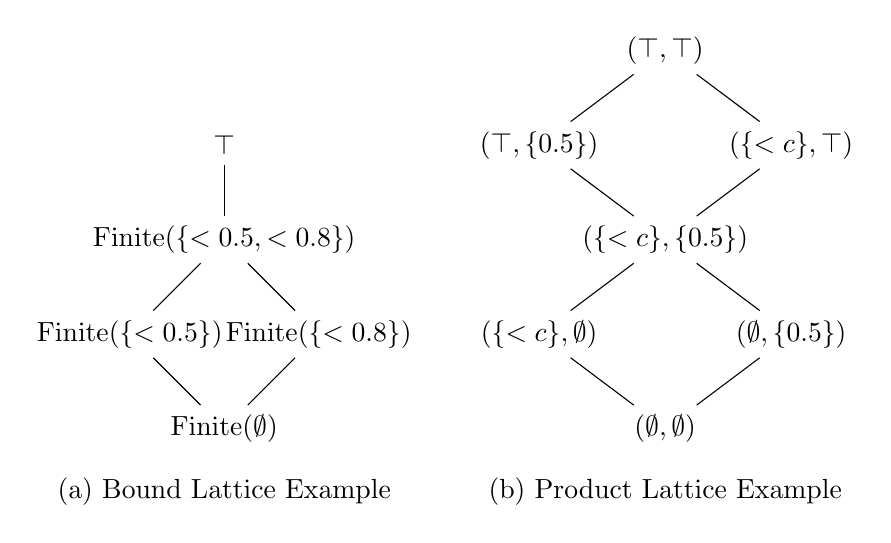
\begin{tikzpicture}[scale=0.8]
  % Individual lattice (left)
  \node (bot1) at (0,0) {$\text{Finite}(\emptyset)$};
  \node (s1) at (-1.5,1.5) {$\text{Finite}(\{<0.5\})$};
  \node (s2) at (1.5,1.5) {$\text{Finite}(\{<0.8\})$};
  \node (s12) at (0,3) {$\text{Finite}(\{<0.5, <0.8\})$};
  \node (top1) at (0,4.5) {$\top$};
  
  \draw (bot1) -- (s1);
  \draw (bot1) -- (s2);
  \draw (s1) -- (s12);
  \draw (s2) -- (s12);
  \draw (s12) -- (top1);
  
  \node at (0,-1) {(a) Bound Lattice Example};
  
  % Product lattice (right)
  \node (bot2) at (7,0) {$(\emptyset, \emptyset)$};
  \node (b1v0) at (5,1.5) {$(\{<c\}, \emptyset)$};
  \node (b0v1) at (9,1.5) {$(\emptyset, \{0.5\})$};
  \node (b1v1) at (7,3) {$(\{<c\}, \{0.5\})$};
  \node (topb) at (5,4.5) {$(\top, \{0.5\})$};
  \node (topv) at (9,4.5) {$(\{<c\}, \top)$};
  \node (top2) at (7,6) {$(\top, \top)$};
  
  \draw (bot2) -- (b1v0);
  \draw (bot2) -- (b0v1);
  \draw (b1v0) -- (b1v1);
  \draw (b0v1) -- (b1v1);
  \draw (b1v1) -- (topb);
  \draw (b1v1) -- (topv);
  \draw (topb) -- (top2);
  \draw (topv) -- (top2);
  
  \node at (7,-1) {(b) Product Lattice Example};
\end{tikzpicture}
\caption{Lattice structure for float types. (a) shows an example bound lattice with comparison bounds. (b) shows the product lattice combining bounds and values.}
\label{fig:lattice}
\end{figure}

The typing rules are as follows:

\begin{mathpar}
    \inferrule[\textsc{Var}]
    {\ }
    {\Gamma, x: \tau \vdash x : \tau}

    \inferrule[\textsc{Let}]
    {\Gamma \vdash e_1 : \tau_1 \\
     \Gamma, x: \tau_1 \vdash e_2 : \tau_2}
    {\Gamma \vdash \letkw \; x = e_1 \; \inkw \; e_2 : \tau_2}

    \inferrule[\textsc{If}]
    {\Gamma \vdash e_1 : \bool \\
     \Gamma \vdash e_2 : \tau \\
     \Gamma \vdash e_3 : \tau}
    {\Gamma \vdash \ifkw \; e_1 \; \thenkw \; e_2 \; \elsekw \; e_3 : \tau}

    \inferrule[\textsc{Float}]
    {\ }
    {\Gamma \vdash c : \float\langle \text{Finite}(\emptyset); \text{Finite}(\{c\}) \rangle}

    \inferrule[\textsc{ContDist}]
    {\ }
    {\Gamma \vdash cdistr : \float\langle \text{Finite}(\emptyset); \top \rangle}

    \inferrule[\textsc{Discrete}]
    {\ }
    {\Gamma \vdash \discrete(p_0, \ldots, p_n) : \intty}

    \inferrule[\textsc{Less}]
    {\Gamma \vdash e : \float\langle B; V \rangle}
    {\Gamma \vdash e < c : \bool}
    \quad \text{where } B \text{ is constrained to include } {<c}

    \inferrule[\textsc{LessEq}]
    {\Gamma \vdash e : \intty}
    {\Gamma \vdash e \leq i : \bool}

    \inferrule[\textsc{Pair}]
    {\Gamma \vdash e_1 : \tau_1 \\
     \Gamma \vdash e_2 : \tau_2}
    {\Gamma \vdash (e_1, e_2) : \tau_1 * \tau_2}

    \inferrule[\textsc{Fst}]
    {\Gamma \vdash e : \tau_1 * \tau_2}
    {\Gamma \vdash \fstkw \; e : \tau_1}

    \inferrule[\textsc{Snd}]
    {\Gamma \vdash e : \tau_1 * \tau_2}
    {\Gamma \vdash \sndkw \; e : \tau_2}

    \inferrule[\textsc{Fun}]
    {\Gamma, x: \tau_1 \vdash e : \tau_2}
    {\Gamma \vdash \funkw \; x \; \rightarrow \; e : \tau_1 \rightarrow \tau_2}

    \inferrule[\textsc{App}]
    {\Gamma \vdash e_1 : \tau_1 \rightarrow \tau_2 \\
     \Gamma \vdash e_2 : \tau_1}
    {\Gamma \vdash e_1 \; e_2 : \tau_2}

    \inferrule[\textsc{True}]
    {\ }
    {\Gamma \vdash \text{true} : \bool}

    \inferrule[\textsc{False}]
    {\ }
    {\Gamma \vdash \text{false} : \bool}

    \inferrule[\textsc{And}]
    {\Gamma \vdash e_1 : \bool \\
     \Gamma \vdash e_2 : \bool}
    {\Gamma \vdash e_1 \&\& e_2 : \bool}

    \inferrule[\textsc{Or}]
    {\Gamma \vdash e_1 : \bool \\
     \Gamma \vdash e_2 : \bool}
    {\Gamma \vdash e_1 || e_2 : \bool}

    \inferrule[\textsc{Not}]
    {\Gamma \vdash e : \bool}
    {\Gamma \vdash \text{not}\; e : \bool}

    \inferrule[\textsc{Unit}]
    {\ }
    {\Gamma \vdash () : \text{unit}}

    \inferrule[\textsc{FinConst}]
    {0 \leq k < n}
    {\Gamma \vdash k\#n : \text{fin}(n)}

    \inferrule[\textsc{FinLess}]
    {\Gamma \vdash e_1 : \text{fin}(n) \\
     \Gamma \vdash e_2 : \text{fin}(n)}
    {\Gamma \vdash e_1 <\#n\; e_2 : \bool}

    \inferrule[\textsc{FinLessEq}]
    {\Gamma \vdash e_1 : \text{fin}(n) \\
     \Gamma \vdash e_2 : \text{fin}(n)}
    {\Gamma \vdash e_1 \leq\#n\; e_2 : \bool}

    \inferrule[\textsc{Observe}]
    {\Gamma \vdash e : \bool}
    {\Gamma \vdash \text{observe}\; e : \text{unit}}

    \inferrule[\textsc{Seq}]
    {\Gamma \vdash e_1 : \tau_1 \\
     \Gamma \vdash e_2 : \tau_2}
    {\Gamma \vdash e_1; e_2 : \tau_2}

    \inferrule[\textsc{Fix}]
    {\Gamma, f: \tau_1 \rightarrow \tau_2, x: \tau_1 \vdash e : \tau_2}
    {\Gamma \vdash \text{fix}\; f\; x := e : \tau_1 \rightarrow \tau_2}

    \inferrule[\textsc{Nil}]
    {\ }
    {\Gamma \vdash \text{nil} : \text{list}(\tau)}

    \inferrule[\textsc{Cons}]
    {\Gamma \vdash e_1 : \tau \\
     \Gamma \vdash e_2 : \text{list}(\tau)}
    {\Gamma \vdash e_1 :: e_2 : \text{list}(\tau)}

    \inferrule[\textsc{Match}]
    {\Gamma \vdash e : \text{list}(\tau_1) \\
     \Gamma \vdash e_1 : \tau_2 \\
     \Gamma, h: \tau_1, t: \text{list}(\tau_1) \vdash e_2 : \tau_2}
    {\Gamma \vdash \text{match}\; e\; \text{with}\; \text{nil} \rightarrow e_1 \mid h :: t \rightarrow e_2\; \text{end} : \tau_2}

    \inferrule[\textsc{Ref}]
    {\Gamma \vdash e : \tau}
    {\Gamma \vdash \text{ref}\; e : \text{ref}(\tau)}

    \inferrule[\textsc{Deref}]
    {\Gamma \vdash e : \text{ref}(\tau)}
    {\Gamma \vdash !e : \tau}

    \inferrule[\textsc{Assign}]
    {\Gamma \vdash e_1 : \text{ref}(\tau) \\
     \Gamma \vdash e_2 : \tau}
    {\Gamma \vdash e_1 := e_2 : \text{unit}}
\end{mathpar}

\section{Type Inference}\label{sec:type-inference}

Type inference for \Slice{} aims to assign a type (e.g., \bool{}, \intty, $\text{fin}(n)$, \float$\langle \dots \rangle$, $\tau_1 * \tau_2$, $\tau_1 \rightarrow \tau_2$, $\text{unit}$, $\text{list}(\tau)$, $\text{ref}(\tau)$) to every subexpression while simultaneously collecting all relevant comparison threshold points for each float expression. This process works by traversing the abstract syntax tree (AST) of the program and generating type constraints based on the structure of the code and the typing rules.

To manage the constraints on float types $\float\langle B; V \rangle$, we maintain two separate ``bags'' for each float expression:
\begin{itemize}
    \item The \emph{bound bag} $B$ collects comparison bounds (e.g., $<0.5$, $\leq 1.2$) from all comparison sites where the expression is used
    \item The \emph{value bag} $V$ tracks concrete float values that the expression can evaluate to
\end{itemize}

Both bags start at the bottom of their respective lattices and are updated through constraint propagation during type inference. 

We have two different kinds of constraints:
\begin{description}
    \item[Type constraints:] types $\tau=\tau'$ being equal.
    \item[Bag constraints:] bags $B=B'$ being equal or $c \in B$ being a member of bag $B$.
\end{description}

Constraints are generated as follows:
\begin{itemize}
    \item In an $\ifkw \; e_1\; \thenkw \; e_2\; \elsekw \; e_3$ expression, $e_1$ must have type \bool, and the types inferred for $e_2$ and $e_3$ must be equal
    \item A comparison $e < c$ requires $e$ to have a $\float\langle B; V \rangle$ type. The comparison adds the bound $<c$ to the bound bag $B$. If $c$ is a constant expression, its value is also tracked in its own value bag.
    \item A comparison $e \leq i$ requires $e$ to have an $\intty$ type.
    \item A $\letkw \; x = e_1 \; \inkw \; e_2$ expression requires the type inferred for $e_1$ to be used for the variable $x$ when inferring the type of $e_2$.
    \item A continuous distribution sampling expression has type $\float\langle B; V \rangle$ where $B$ starts as $\text{Finite}(\emptyset)$ and $V$ is $\top$ (since it can produce any value in its range).
    \item A $\discrete(p_0, \ldots, p_n)$ expression has type $\intty$, representing an integer in the range $[0,n]$ with probability distribution given by the probabilities.
    \item A pair $(e_1, e_2)$ has type $\tau_1 * \tau_2$ if $e_1$ has type $\tau_1$ and $e_2$ has type $\tau_2$.
    \item For $\fstkw \; e$, $e$ must have a pair type $\tau_1 * \tau_2$, and the result has type $\tau_1$.
    \item For $\sndkw \; e$, $e$ must have a pair type $\tau_1 * \tau_2$, and the result has type $\tau_2$.
    \item For $\funkw \; x \; \rightarrow \; e$, if $e$ has type $\tau_2$ under the assumption that $x$ has type $\tau_1$, then the function has type $\tau_1 \rightarrow \tau_2$.
    \item For $e_1 \; e_2$, $e_1$ must have a function type $\tau_1 \rightarrow \tau_2$, and $e_2$ must have type $\tau_1$. The result has type $\tau_2$.
    \item Boolean constants $\text{true}$ and $\text{false}$ have type \bool.
    \item Boolean operations ($\&\&$, $||$, $\text{not}$) require their operands to have type \bool{} and return type \bool.
    \item The unit value $()$ has type $\text{unit}$.
    \item A finite constant $k\#n$ has type $\text{fin}(n)$ if $0 \leq k < n$.
    \item Finite comparisons $e_1 <\#n\; e_2$ and $e_1 \leq\#n\; e_2$ require both operands to have type $\text{fin}(n)$ and return type \bool.
    \item $\text{observe}\; e$ requires $e$ to have type \bool{} and returns type $\text{unit}$.
    \item For $e_1; e_2$, the result has the type of $e_2$.
    \item For $\text{fix}\; f\; x := e$, if $e$ has type $\tau_2$ under the assumptions that $f$ has type $\tau_1 \rightarrow \tau_2$ and $x$ has type $\tau_1$, then the result has type $\tau_1 \rightarrow \tau_2$.
    \item $\text{nil}$ can have type $\text{list}(\tau)$ for any type $\tau$.
    \item For $e_1 :: e_2$, if $e_1$ has type $\tau$ and $e_2$ has type $\text{list}(\tau)$, the result has type $\text{list}(\tau)$.
    \item For list pattern matching, the scrutinee must have type $\text{list}(\tau_1)$, and both branches must have the same type $\tau_2$.
    \item For $\text{ref}\; e$, if $e$ has type $\tau$, the result has type $\text{ref}(\tau)$.
    \item For $!e$, if $e$ has type $\text{ref}(\tau)$, the result has type $\tau$.
    \item For $e_1 := e_2$, $e_1$ must have type $\text{ref}(\tau)$ and $e_2$ must have type $\tau$. The result has type $\text{unit}$.
\end{itemize}

Bag constraint solving is implemented using a variant of the disjoint-set data structure, commonly known as union-find.
A union-find data structure maintains a collection of disjoint sets (our bags). Each bag is represented by a tree, where the root is the canonical representative of the set. It supports three main operations:
\begin{itemize}
    \item \texttt{find(b)}: Returns the canonical representative (root) of the bag $b$, containing the set of threshold points currently known for $b$. Path compression is used for efficiency: during the traversal from $b$ to the root, all nodes encountered are made direct children of the root. This flattens the tree and speeds up future \texttt{find} operations.
    \item \texttt{union(b1, b2)}: Merges the bags containing $b1$ and $b2$. It first finds the roots of both bags. If they are different, one root is made a child of the other. Crucially, when merging bags associated with \float{} types, the sets of threshold points stored at the roots are combined (using set union).
    \item \texttt{add(b, c)}: Adds a new threshold point $c$ to the bag $b$.
\end{itemize}

Type constraints are solved using unification. When two types $t_1$ and $t_2$ must be unified:
\begin{itemize}
    \item If $t_1 = \bool$ and $t_2 = \bool$, unification succeeds.
    \item If $t_1 = \intty$ and $t_2 = \intty$, unification succeeds.
    \item If $t_1 = \text{unit}$ and $t_2 = \text{unit}$, unification succeeds.
    \item If $t_1 = \text{fin}(n)$ and $t_2 = \text{fin}(m)$, unification succeeds if $n = m$.
    \item If $t_1 = \float\langle B_1; V_1 \rangle$ and $t_2 = \float\langle B_2; V_2 \rangle$, we must unify both components:
        \begin{itemize}
            \item Bound bags: $B_1$ and $B_2$ are unified to ensure both expressions share the same comparison context
            \item Value bags: $V_1 \sqcup V_2$ is computed to combine value information
        \end{itemize}
    \item If $t_1 = \tau_{1a} * \tau_{1b}$ and $t_2 = \tau_{2a} * \tau_{2b}$, unification succeeds if $\tau_{1a}$ unifies with $\tau_{2a}$ and $\tau_{1b}$ unifies with $\tau_{2b}$.
    \item If $t_1 = \tau_{1a} \rightarrow \tau_{1b}$ and $t_2 = \tau_{2a} \rightarrow \tau_{2b}$, unification succeeds if $\tau_{1a}$ unifies with $\tau_{2a}$ and $\tau_{1b}$ unifies with $\tau_{2b}$.
    \item If $t_1 = \text{list}(\tau_1)$ and $t_2 = \text{list}(\tau_2)$, unification succeeds if $\tau_1$ unifies with $\tau_2$.
    \item If $t_1 = \text{ref}(\tau_1)$ and $t_2 = \text{ref}(\tau_2)$, unification succeeds if $\tau_1$ unifies with $\tau_2$.
    \item If the types are incompatible (e.g., \bool{} and \float{}, \intty{} and \float{}, pair and function), a type error occurs. Meta-variables (placeholder types) are handled by instantiation during unification.
\end{itemize}

The inference algorithm recursively walks the expression AST. It maintains an environment mapping variables to their inferred types. At each node, it generates and solves constraints using unification and the bag operations. The final result is an AST annotated with types, where each $\float\langle B; V \rangle$ type carries both bags populated with the relevant bounds and values determined by the inference process.

\section{Discretization}\label{sec:discretization}

After type inference, we have a \Slice{} expression annotated with types, where each $\float\langle B; V \rangle$ type includes:
\begin{itemize}
    \item A bound bag $B$ containing all comparison bounds (e.g., $<0.5$, $\leq 1.2$)
    \item A value bag $V$ containing known constant values or $\top$
\end{itemize}

The discretization process uses the bound bag $B$ to determine how to partition continuous distributions. For each continuous distribution with type $\float\langle B; V \rangle$, we extract the numeric thresholds from $B$ to create discretization intervals.

The core idea is to map the continuous range of a float variable onto a finite set of integers, representing intervals defined by the threshold points in its bag. A comparison against a threshold constant $c_k$ becomes a comparison against the corresponding interval index $k$.

Let $e$ be a subexpression with inferred type $\float\langle B; V \rangle$. From the bound bag $B$, we extract the set of numeric thresholds $\{c_0, \dots, c_n\}$ (sorting and removing duplicates from bounds like $<c_i$ and $\leq c_i$). Let $\texttt{discretize}(e)$ be the corresponding discretized expression.

\begin{itemize}
    \item \textbf{Continuous Distribution}: If $e = cdistr$ with type $\float\langle B; V \rangle$, we extract threshold points $\{c_0, \dots, c_n\}$ from the bound bag $B$. We define $n+1$ intervals based on these points: $I_0 = (-\infty, c_0)$, $I_1 = [c_0, c_1)$, \dots, $I_n = [c_{n-1}, c_n)$, $I_{n+1} = [c_n, +\infty)$. The discretization is $\texttt{discretize}(e) = \discrete(p_0, \dots, p_{n+1})$, where $p_i$ is the probability mass of the original continuous distribution $cdistr$ within the interval $I_i$. This is calculated using the Cumulative Distribution Function (CDF) of the specific distribution:
    \[ p_i = \text{CDF}(\text{right}_i) - \text{CDF}(\text{left}_i) \]
    where $\text{left}_i$ and $\text{right}_i$ are the bounds of interval $I_i$ (using $-\infty$ and $+\infty$ appropriately). This \discrete{} distribution yields an integer $i$ with probability $p_i$, signifying that the original continuous value fell within interval $I_i$. Special handling is needed for degenerate cases (e.g., zero-width intervals for uniform).

    \item \textbf{Discrete Distribution}: If $e = \discrete(p_0, \ldots, p_n)$ with type $\intty$, the discretization simply preserves the discrete distribution as is: $\texttt{discretize}(e) = \discrete(p_0, \ldots, p_n)$. This expression returns an integer value $i \in \{0, 1, \ldots, n\}$ with probability $p_i$.

    \item \textbf{Less Than Comparison}: If $e = e' < c_k$, where $e'$ has type $\float\langle B; V \rangle$. We extract the sorted threshold set $\{c_0, \dots, c_n\}$ from the bound bag $B$, and $c_k$ is the $k$-th smallest element in this set. The discretization is $\texttt{discretize}(e) = \texttt{discretize}(e') \leq k$. The discretized subexpression $\texttt{discretize}(e')$ evaluates to an integer $i$ representing an interval $I_i$. The comparison $i \leq k$ checks if the value falls into any of the intervals $I_0, \dots, I_k$. The union of these intervals is $(-\infty, c_k)$. Thus, the comparison correctly determines if the original value of $e'$ was less than $c_k$.

    \item \textbf{Less Than or Equal Comparison}: If $e = e' \leq i$, where $e'$ has type $\intty$, the discretization preserves the comparison: $\texttt{discretize}(e) = \texttt{discretize}(e') \leq i$. This form is used for comparing integer values, particularly the results of discrete distributions.

    \item \textbf{Variables, Let, If, Pairs, Projections, Functions, Application}: These constructs are translated recursively, preserving their structure:
    \begin{itemize}
        \item $\texttt{discretize}(x) = x$
        \item $\texttt{discretize}(\letkw \; x = e_1 \; \inkw \; e_2) = \letkw \; x = \texttt{discretize}(e_1) \; \inkw \; \texttt{discretize}(e_2)$
        \item $\texttt{discretize}(\ifkw \; e_1 \; \thenkw \; e_2 \; \elsekw \; e_3) = \ifkw \; \texttt{discretize}(e_1) \; \thenkw \; \texttt{discretize}(e_2) \; \elsekw \; \texttt{discretize}(e_3)$
        \item $\texttt{discretize}((e_1, e_2)) = (\texttt{discretize}(e_1), \texttt{discretize}(e_2))$
        \item $\texttt{discretize}(\fstkw \; e) = \fstkw \; (\texttt{discretize}(e))$
        \item $\texttt{discretize}(\sndkw \; e) = \sndkw \; (\texttt{discretize}(e))$
        \item $\texttt{discretize}(\funkw \; x \; \rightarrow \; e) = \funkw \; x \; \rightarrow \; (\texttt{discretize}(e))$
        \item $\texttt{discretize}(e_1 \; e_2) = \texttt{discretize}(e_1) \; \texttt{discretize}(e_2)$
    \end{itemize}

    \item \textbf{Boolean, Unit, Finite Constants}: These are already discrete and pass through unchanged.
    \item \textbf{Finite Comparisons}: Comparisons like $e_1 <\#n\; e_2$ are preserved as-is since they already operate on discrete finite types.
    \item \textbf{Lists, References, Boolean Operations}: These constructs are translated recursively, preserving their structure.
\end{itemize}

This process effectively translates continuous distributions into discrete distributions based on the thresholds used in the program, while preserving the original discrete distributions and program structure, including functional constructs, pairs, lists, references, and finite types.

\section{Soundness Proof}\label{sec:soundness}


\section{Implementation}\label{sec:implementation}

We have implemented \Slice{} as an OCaml-based compiler that transforms continuous probabilistic programs into discrete ones, which can then be analyzed using exact inference engines. The implementation consists of two main components: the \Slice{} compiler (\texttt{cdice}) and the Dice inference engine~\cite{Holtzen2020Dice}.

\subsection{Architecture Overview}

Figure~\ref{fig:architecture} shows the overall architecture of the \Slice{} system.

\begin{figure}[h]
\centering
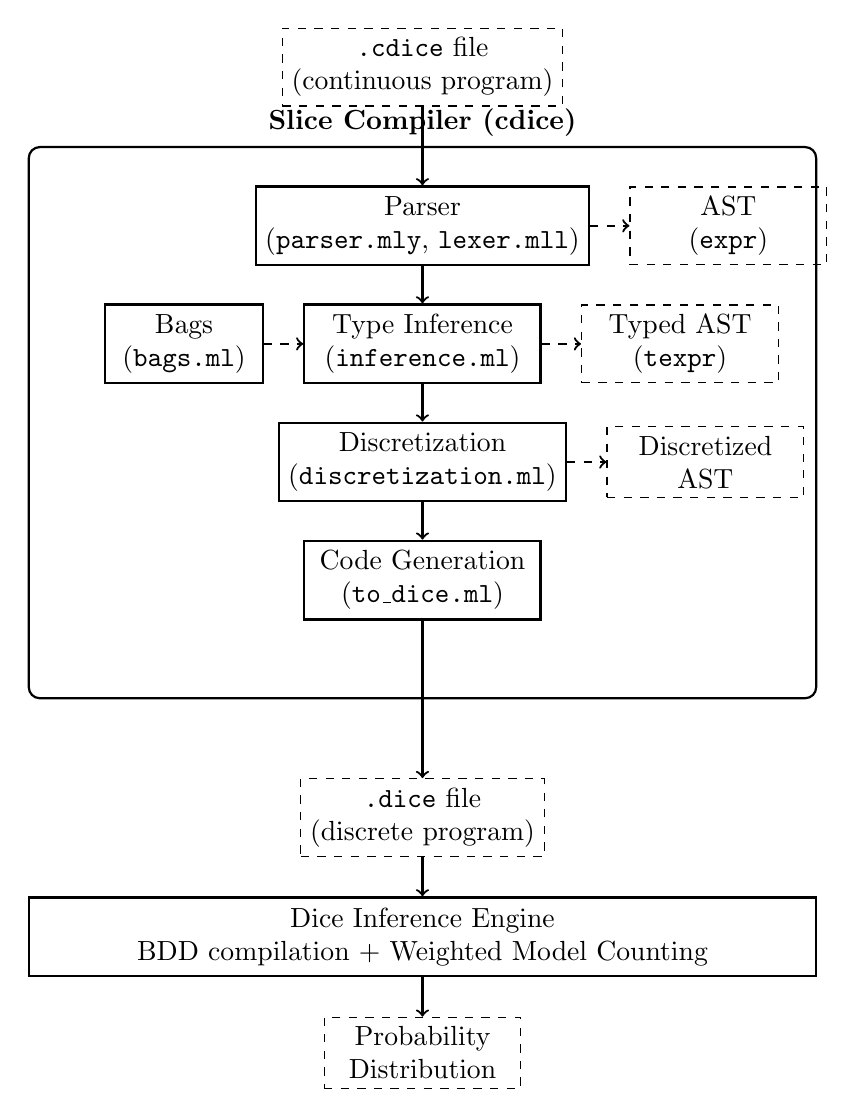
\begin{tikzpicture}[
    node distance=1.5cm,
    component/.style={rectangle, draw, thick, minimum width=3cm, minimum height=1cm, align=center},
    data/.style={rectangle, draw, dashed, minimum width=2.5cm, minimum height=0.8cm, align=center},
    arrow/.style={->, thick},
    bigbox/.style={draw, thick, rounded corners, inner sep=0.3cm}
]
    % Input
    \node[data] (input) {\texttt{.cdice} file\\(continuous program)};
    
    % Slice compiler box
    \node[bigbox, below=0.5cm of input, minimum width=10cm, minimum height=7cm] (slicebox) {};
    \node[above] at (slicebox.north) {\textbf{\Slice{} Compiler (cdice)}};
    
    % Components inside Slice
    \node[component, below=1cm of input] (parser) {Parser\\(\texttt{parser.mly}, \texttt{lexer.mll})};
    \node[component, below of=parser] (typeinf) {Type Inference\\(\texttt{inference.ml})};
    \node[component, below of=typeinf] (disc) {Discretization\\(\texttt{discretization.ml})};
    \node[component, below of=disc] (todice) {Code Generation\\(\texttt{to\_dice.ml})};
    
    % Intermediate data structures
    \node[data, right=0.5cm of parser] (ast) {AST\\(\texttt{expr})};
    \node[data, right=0.5cm of typeinf] (tast) {Typed AST\\(\texttt{texpr})};
    \node[data, right=0.5cm of disc] (dast) {Discretized\\AST};
    
    % Bags module
    \node[component, left=0.5cm of typeinf, minimum width=2cm] (bags) {Bags\\(\texttt{bags.ml})};
    
    % Output from Slice
    \node[data, below=1cm of slicebox] (dice) {\texttt{.dice} file\\(discrete program)};
    
    % Dice engine
    \node[component, below=0.5cm of dice, minimum width=10cm] (diceengine) {Dice Inference Engine\\BDD compilation + Weighted Model Counting};
    
    % Final output
    \node[data, below=0.5cm of diceengine] (output) {Probability\\Distribution};
    
    % Arrows
    \draw[arrow] (input) -- (parser);
    \draw[arrow] (parser) -- (typeinf);
    \draw[arrow] (typeinf) -- (disc);
    \draw[arrow] (disc) -- (todice);
    \draw[arrow] (todice) -- (dice);
    \draw[arrow] (dice) -- (diceengine);
    \draw[arrow] (diceengine) -- (output);
    
    % Side arrows for data structures
    \draw[arrow, dashed] (parser) -- (ast);
    \draw[arrow, dashed] (typeinf) -- (tast);
    \draw[arrow, dashed] (disc) -- (dast);
    \draw[arrow, dashed] (bags) -- (typeinf);
\end{tikzpicture}
\caption{Architecture of the \Slice{} system. The \Slice{} compiler transforms continuous probabilistic programs into discrete ones through type-directed discretization. The resulting discrete program is then processed by the Dice inference engine to compute exact probability distributions.}
\label{fig:architecture}
\end{figure}

\subsection{Implementation Details}

\paragraph{Parser and Lexer} The frontend uses OCaml's Menhir parser generator to parse \texttt{.cdice} source files. The parser (\texttt{parser.mly}) defines the concrete syntax and produces an abstract syntax tree (AST) represented by the \texttt{expr} type. The lexer (\texttt{lexer.mll}) handles tokenization, including special tokens for finite type comparisons (e.g., \texttt{<\#n}).

\paragraph{Type Inference} The type inference module (\texttt{inference.ml}) implements the two-bag type system described in Section~\ref{sec:type-inference}. It uses a constraint-based approach with unification to infer types while collecting comparison bounds. The implementation features:
\begin{itemize}
    \item A union-find data structure for managing bags efficiently
    \item Listener patterns for propagating constraints between related expressions
    \item Subtyping rules that ensure proper information flow
\end{itemize}

\paragraph{Bags Module} The \texttt{bags.ml} module provides the lattice-based data structures for tracking bounds and values. It implements:
\begin{itemize}
    \item Generic bag operations (union, equality checking)
    \item Specialized \texttt{BoundBag} for comparison bounds ($<c$, $\leq c$)
    \item \texttt{FloatBag} for tracking concrete float values
    \item Efficient representation using either finite sets or $\top$
\end{itemize}

\paragraph{Discretization} The discretization module (\texttt{discretization.ml}) transforms typed continuous programs into discrete ones. For each continuous distribution, it:
\begin{enumerate}
    \item Extracts comparison thresholds from the bound bag
    \item Computes interval probabilities using distribution CDFs
    \item Generates equivalent discrete distributions
    \item Transforms comparisons to operate on interval indices
\end{enumerate}

\paragraph{Code Generation} The \texttt{to\_dice.ml} module generates Dice source code from the discretized AST. It handles the translation of \Slice{} constructs to their Dice equivalents, including special handling for finite types that become integers in Dice.

\paragraph{Runtime and Evaluation} The implementation includes:
\begin{itemize}
    \item An interpreter (\texttt{interp.ml}) for sampling-based execution
    \item Statistical testing to verify discretization correctness
    \item Support for multiple output formats (Dice, SPPL)
\end{itemize}

\subsection{Integration with Dice}

The Dice inference engine~\cite{Holtzen2020Dice} provides exact inference for discrete probabilistic programs using Binary Decision Diagrams (BDDs) and weighted model counting. Our discretized programs are designed to work seamlessly with Dice's capabilities:
\begin{itemize}
    \item Discrete distributions map directly to Dice's \texttt{discrete} construct
    \item Finite types become bounded integers
    \item Observations translate to Dice's conditioning primitives
\end{itemize}

The complete workflow is automated through the \texttt{run\_contdice.sh} script, which pipes the output of \Slice{} directly to Dice for inference.

\subsection{Engineering Considerations}

The implementation prioritizes correctness and clarity:
\begin{itemize}
    \item Extensive use of OCaml's type system for safety
    \item Modular design allowing independent testing of components
    \item Clear separation between syntax-directed and semantic phases
    \item Comprehensive test suite including adversarial examples
\end{itemize}

The system is open-source and available at \url{https://github.com/[repository-url]}, along with benchmarks and documentation.


\section{Evaluation}\label{sec:evaluation}


\subsection{Synthetic benchmarks}\label{sec:synthetic-benchmarks}
- Describe the benchmarks, the structure they have
- Scaling graphs
- Divide cdice and Dice

* We compare all benchmarks that sppl runs on
\subsection{Psi benchmarks}\label{sec:psi-benchmarks}
- describe benchmarks, cite paper
- simplications we made such as expanding out arrays
- graphs (cdice + dice vs sppl vs bitblast)

\subsection{Fairness benchmarks}\label{sec:fairness-benchmarks}
- describe benchmarks, cite paper
- simplications we made such as expanding out arrays
- graphs (cdice + dice vs sppl vs bitblast)





\section{Related Work}
\label{sec:related}

\paragraph{Discrete-only probabilistic languages}  
Several recent systems achieve \emph{exact inference} by restricting models to finite, discrete random variables. \emph{Roulette} extends Racket with first-class support for finitely-supported distributions and leverages symbolic evaluation to compile queries into weighted model-counting problems, enabling scalable exact conditioning on complex programs~\cite{Moy2025Roulette}. \emph{Dice} follows a similar philosophy in an OCaml DSL, compiling discrete programs to weighted model counting to perform exact Bayesian updates even on thousands of Boolean and finite-categorical variables~\cite{Holtzen2020Dice}. Earlier work in probabilistic logic programming, most prominently \emph{ProbLog}, annotates Prolog facts with probabilities and reduces inference to weighted Boolean formulas that can likewise be solved exactly~\cite{DeRaedt2007ProbLog}. These languages demonstrate the power of exact reasoning, but by construction they \emph{cannot express continuous random quantities}; consequently they offer no built-in path for analysing models that naturally mix real-valued and discrete structure.  

\paragraph{Symbolic treatment of mixed models}  
\emph{SPPL} occupies an intermediate point on the design spectrum. By enforcing syntactic restrictions that guarantee every program can be translated into a finite \emph{sum-product expression}, SPPL supports models with both discrete and continuous components while still admitting \emph{symbolic} exact inference~\cite{Saad2021SPPL}. Rather than discretising the continuous parts, SPPL derives closed-form integrals when possible; exactness is retained for a narrow class of models. There is no mechanism for turning the remaining continuous structure into a discrete program that could reuse the powerful inference back-ends of Dice, Roulette, or ProbLog.

\paragraph{Continuous and hybrid PPLs with approximate inference}  
The majority of widely-used PPLs treat \emph{continuous} distributions as first-class and rely on approximate inference. Systems such as \emph{Stan} (C++), \emph{PyMC} (Python), \emph{Pyro} (Python on PyTorch), \emph{TensorFlow Probability} and its precursor \emph{Edward} expose rich continuous distributions and obtain posteriors with Hamiltonian Monte Carlo, variational inference, or sequential Monte Carlo~\cite{Carpenter2017Stan,Salvatier2016PyMC3,Bingham2019Pyro,Dillon2017TFP,Tran2016Edward}. These frameworks deliver high accuracy for differentiable densities but can struggle with discrete latent structure or discontinuities that arise after naïve discretisation. Crucially, none of them offers an automated pathway to convert continuous sub-expressions into discrete replacements that would make exact inference feasible.

\paragraph{Universal languages supporting both regimes}  
Universal or ``hybrid'' languages aim for expressiveness by embedding probabilistic primitives into general-purpose hosts. \emph{Anglican} (Clojure), \emph{WebPPL} (JavaScript), \emph{Figaro} (Scala) and \emph{Infer.NET} (C\#) permit arbitrary mixtures of discrete and continuous variables with inference based on importance sampling, Gibbs, expectation propagation, or lightweight MCMC~\cite{Tolpin2016Anglican,Goodman2014WebPPL,Pfeffer2009Figaro,Minka2018InferNET}. More recently, Julia-based systems such as \emph{Turing.jl} and \emph{Gen.jl} expose programmable inference interfaces, while \emph{Bean Machine} offers a declarative syntax atop PyTorch~\cite{Ge2018Turing,CusumanoTowner2019Gen,Tehrani2020BeanMachine}. Classic languages like \emph{Church} pioneered the ``evaluation-as-sampling'' view that underlies many of these systems~\cite{Goodman2008Church}. Discretization transformations are left entirely to the user and are not integrated with the inference engine.

\jules{Talk about Steven's abstract interpretation work here}

\paragraph{Positioning of our work}  
Our contribution lies precisely at the intersection left open by the above lines of research. We propose a \emph{language-level transformation} that automatically discretises continuous sub-programs while preserving the semantics required for exact Bayesian reasoning in the discrete fragment. When discretization successfully translates all continuous distributions, we can translate the program into the finite domain accepted by Dice (or Roulette, or ProbLog), and inherit their fast exact inference without sacrificing the modelling convenience of continuous distributions. 
Empirically, our approach of discretizing programs and running them through Dice's inference engine achieves significantly faster runtimes compared to SPPL's symbolic methods, while maintaining exactness. Unlike continuous PPLs that settle for stochastic approximations, our approach bridges the gap between expressive modelling and fast exact computation. Partial discretization is also possible, and could be used to speed up inference without sacrificing expressiveness.

\medskip  
In summary, existing discrete PPLs excel at exactness but lack continuous support, symbolic languages like SPPL require restrictive structure and are slower than model counting approaches, and continuous or hybrid frameworks favour approximate inference. To our knowledge none of these systems automates the conversion of continuous programs into a discrete representation amenable to exact inference; our work addresses precisely that missing piece.

\paragraph{Future work}
In the future, we would like to extend our work to symbolically integrate tractable combinations of continous distributions beyond the cumulative distribution function.
We would also like to improve mixed continuous-discrete inference by partial discretization, summing out the discrete variables using weighted model counting techniques, and running the remaining continuous inference using standard continuous inference techniques.

\bibliographystyle{ACM-Reference-Format}
\bibliography{refs}



\end{document}

